\documentclass{article}
\usepackage[T1]{fontenc}
\usepackage{lmodern}
\usepackage{graphicx}
\usepackage{amsmath,amssymb}
\usepackage[a4paper,margin=2cm]{geometry}
\usepackage[absolute,overlay]{textpos}
\setlength{\TPHorizModule}{1mm}
\setlength{\TPVertModule}{1mm}
\usepackage[indonesian]{babel}
\usepackage{hyperref}
\setlength{\emergencystretch}{2em}
% unit: Halaman 37

\begin{document}

% === Halaman 37 (llm) ===

\vspace{32.08mm}

\begin{itemize}
    \item Hasil enkripsi seluruhnya adalah sebagai berikut:

    \begin{tabular}{ll}
        Plainteks & : terimapesanangulaikambing \\
        Kunci & : soreangsoreangsoreangsore \\
        Cipherteks & : LSIMMNVWGRRAAMMZRMKNSTWEK
    \end{tabular}

    \item Tanpa menggunakan \textit{Vigenere Square} pun enkripsi tetap dapat dihitung secara \textit{Caesar Cipher} dengan menjumlahkan plainteks $p_j$ dengan kunci $k_i$ dalam modulus 26:

    \begin{align*}
        \text{Enkripsi: } & c_j = E(p_j) = (p_j + k_i) \pmod{26} \tag{1} \\
        \text{Dekripsi: } & p_j = D(c_j) = (c_j - k_i) \pmod{26} \tag{2}
    \end{align*}

    Contoh:
    \[ (t + s) \pmod{26} = (19 + 18) \pmod{26} = 37 \pmod{26} = 11 = L \]
    \[ (e + o) \pmod{26} = (4 + 14) \pmod{26} = 18 \pmod{26} = 18 = S, \text{ dst} \]
\end{itemize}

% deskripsi: Kotak referensi pemetaan huruf alfabet ke angka dari A=0 sampai Z=25
% bbox normalisasi: [0.5320, 0.0080, 0.9860, 0.1160]
\begin{textblock*}{95.34mm}(111.72mm,2.38mm)
\noindent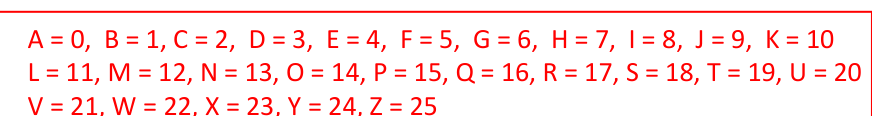
\includegraphics[width=95.34mm,height=32.08mm]{../../images/llm/page_037_img_01.png}%
\end{textblock*}

\end{document}
